%%=============================================================================%
%% 设置论文格式（学位、盲评、Adobe 字体）
%%-----------------------------------------------------------------------------%
%% 博士、正常版本、不使用 Adobe 字体
%% \documentclass[lang=chs, degree=phd, blindreview=false, adobe=false]{yanputhesis}
%% 博士、盲评版本、不使用 Adobe 字体
%% \documentclass[lang=chs, degree=phd, blindreview=true, adobe=false]{yanputhesis}
%% 博士、正常版本、强制使用 Windows 系统字体
% \documentclass[lang=chs, degree=phd, blindreview=false, winfonts=true]{yanputhesis}
%% 硕士、正常版本、不使用 Adobe 字体
% \documentclass[lang=chs, degree=master, blindreview=false, winfonts=true]{yanputhesis}
%% 硕士、盲评版本、不使用 Adobe 字体
%% \documentclass[lang=chs, degree=master, blindreview=true, adobe=false]{yanputhesis}

% \documentclass[lang=chs, degree=master, blindreview=true, winfonts=true, academic=true]{yanputhesis} % 盲审
\documentclass[lang=chs, degree=master, blindreview=false, winfonts=true, academic=true]{yanputhesis}  % 非盲审

%%=============================================================================%
%% 导言区：请自行添加额外宏包
%%-----------------------------------------------------------------------------%
\usepackage{blindtext}                                      % 生成无意义文本
\usepackage{metalogo}                                       % 软件标志
% \usepackage[binary-units=true]{siunitx}                     % 物理量单位
\usepackage{siunitx}
\usepackage{amsmath}                                        % 基础数学库
\usepackage{ifplatform}
\usepackage{eso-pic}                                       % 页面背景图
\windowstrue   % 声明是 Windows

%%=============================================================================%
%% 图片占位框开关（不加载图像内容，但保留原尺寸与排版）
%%-----------------------------------------------------------------------------%
\newif\ifdraftfigures
% \draftfigurestrue            % 占位模式：true=空白框
\draftfiguresfalse             % 占位模式：false=正常加载图片
\ifdraftfigures
    \setkeys{Gin}{draft}
\fi

%%=============================================================================%
%% 版本控制配置
%%-----------------------------------------------------------------------------%
%% 设置当前使用的版本目录名
%% 通过修改这个变量轻松切换不同版本
%% Thesis_v1_20250901, Thesis_v2_20251101 等
\newcommand{\VersionControl}{Thesis_v1_20250901}        % 当前版本
\newcommand{\VersionDate}{2025-09-01}                      % 版本日期  
\newcommand{\VersionDescription}{模块化版本控制结构}        % 版本描述
%% 版本说明：
%% v1_20250901 - 初始模块化版本，包含完整的章节结构
%% v2_20251101 - [预留给未来版本使用]
%% v3_20251201 - [预留给未来版本使用]
%%=============================================================================%
%% 基本信息录入
%%-----------------------------------------------------------------------------%
\title{基于 LaTeX 排版的 \\ 西北工业大学论文模板}{          % 中英文标题
    Yet Another Thesis Template of \\ Northwestern Polytechnical University
}                                                           % 请自行断行
\author{\blindreview{张三丰}}{\blindreview{Sanfeng Zhang}}  % 姓名（添加盲评标记）
\date{2026年3月}{March 2026}                                          % 盲审日期
\school{电子信息学院}{School of Electronics and Information}          % 学院
\major{信息与通信工程}{Information and Communication Engineering}     % 专业 博士请添加 Ph
\advisor{\blindreview{李四海}}{\blindreview{Sihai Li}}      % 导师（添加盲评标记）
\advisorAcademicRank{教授}{Professor}						  % 导师中英学术职位（教授 Professor、副教授 Associate Professor、研究员 Researcher 和讲师 Lecturer）
\studentnumber{2023123456}                                  % 学号
\funding{本研究得到玄学基金（编号23336666）资助。}{         % 基金资助
    The present work is supported by Funding of Metaphysics %
    (Project No：23336666).}                                %
%%=============================================================================%
%% 文档开始
%%-----------------------------------------------------------------------------%
\begin{document}
\AddToShipoutPictureBG*{%
    \AtPageLowerLeft{%
        
\includegraphics[draft=false,width=\paperwidth,height=\paperheight]{Resources/acad_head.jpg}%
    }%
}
%%-----------------------------------------------------------------------------%
%% 总前言，包含封皮页、中英文标题、中英文摘要、目录
%%-----------------------------------------------------------------------------%
\frontmatter                                                % 前言部分
\maketitle                                                  % 封皮页及标题页
%%-----------------------------------------------------------------------------%
\makeCommitteePage{                                         % 学位论文评阅人
    \reviewers{\fullBlindReview{2}}                         % 和答辩委员会名单
    \committee{2026 年 x 月 y 日}{
        \defenseChair{赵xx}{教授}{西北工业大学}
        \committeeMember{周xx}{教授}{西北工业大学}
        \committeeMember{冯xx}{教授}{西北工业大学}
        \defenseSecretary{金xx}{教授}{西北工业大学}
    }
}
%%-----------------------------------------------------------------------------%
%% 中英文摘要（使用版本控制变量动态引入）
%%-----------------------------------------------------------------------------%
\begin{abstract}                                            % 中文摘要开始
    这是在西北工业大学本科毕业设计、硕博研究生毕业论文格式的要求下的一份 LaTeX文档类模板。使用者无需额外修改格式控制细节，直接在所发布的样例基础上，修改章节标题，撰写内容，即可完成毕业设计论文任务。            %
    \begin{keywords}                                        % 中文关键词开始
        学位论文 \sep 模板 \sep \LaTeX                      %
    \end{keywords}                                          % 中文关键词结束
\end{abstract}                                              % 中文摘要结束          % 中文摘要
\input{\VersionControl/abstract/english-abstract}          % 英文摘要
%%-----------------------------------------------------------------------------%
\tableofcontents                                            % 目录
\listoffigures                                              % 图目录（学校未做要求）
\listoftables                                               % 表目录（学校未做要求）
\printnomenclature                                          % 符号表（学校未做要求）
%%=============================================================================%
%% 正文部分（使用版本控制变量动态引入各章节）
%%-----------------------------------------------------------------------------%
\mainmatter
\sDefault

%% 第一章：绪论
\chapter{chapter 01}
\chaptermark{chapter 01}

Attention is all you need \cite{vaswani2017attention}.
\cleardoublepage

%% 第二章：相关理论基础
\chapter{chapter 02}
\chaptermark{chapter 02}

Attention is all you need \cite{vaswani2017attention}.
\cleardoublepage

%% 第三章：主要方法一
\chapter{chapter 03}
\chaptermark{chapter 03}


\cleardoublepage

%% 第四章：主要方法二
\chapter{chapter 04}
\chaptermark{chapter 04}
\cleardoublepage

%% 第五章：总结与展望
\chapter{chapter 05}
\chaptermark{chapter 05}
\cleardoublepage

%%=============================================================================%
%% 参考文献以及附录（使用版本控制变量动态引入）
%%-----------------------------------------------------------------------------%
%% \bibliographystyle{nputhesis}                               % GB/T 7714-2015 格式
\bibliographystyle{nputhesis-noslash}                       % 参考文献改进格式
\bibliography{\VersionControl/references/reference}         % 参考文献（使用版本控制变量）
%% 附录部分
%% 附录部分
\appendix

\chapter{一份说明 顺便测试英文标题 Title}

强烈不推荐英文标题！仅供测试，擅自使用后果自负。

\section{测试附录子标题}

这是一份附录，请放置一些独立的证明、源代码、或其他辅助资料。

\nomenclature{$r$}{圆（或球）的半径}
\nomenclature{$C$}{圆的周长}
\nomenclature{$S$}{圆的面积}

\begin{equation}
    C = 2 \pi r
\end{equation}

\begin{equation}
    S = \pi r^2
\end{equation}

\cleardoublepage

\chapter{另一份说明}

这是另一份附录，请放置一些独立的证明、源代码、或其他辅助资料。

\nomenclature{$S_{\text{sphere}}$}{球的表面积}
\nomenclature{$V_{\text{sphere}}$}{球的体积}

\begin{equation}
    S_{\text{sphere}} = 4 \pi r^2
\end{equation}

\begin{equation}
    V_{\text{sphere}} = \frac43 \pi r^3
\end{equation}

\cleardoublepage         % 附录
%%=============================================================================%
%% 文档附页部分（致谢、参加科研情况、知识产权与原创性声明）
%%-----------------------------------------------------------------------------%
\backmatter                                                 % 文档附页部分
%%-----------------------------------------------------------------------------%
%% 致谢
\begin{acknowledgements}                                    % 致谢开始
    最诚挚的谢意。
\end{acknowledgements}                                      % 致谢结束
   % 致谢
%% 参加科研情况
\begin{accomplishments}                                     % 参加科研情况开始
    [1] AAA

    [2] BBB
\end{accomplishments}                                       % 参加科研情况结束
    % 参加科研情况
%%-----------------------------------------------------------------------------%
% \makestatement                                            % 知识产权与原创性声明（改为插入签字扫描页）
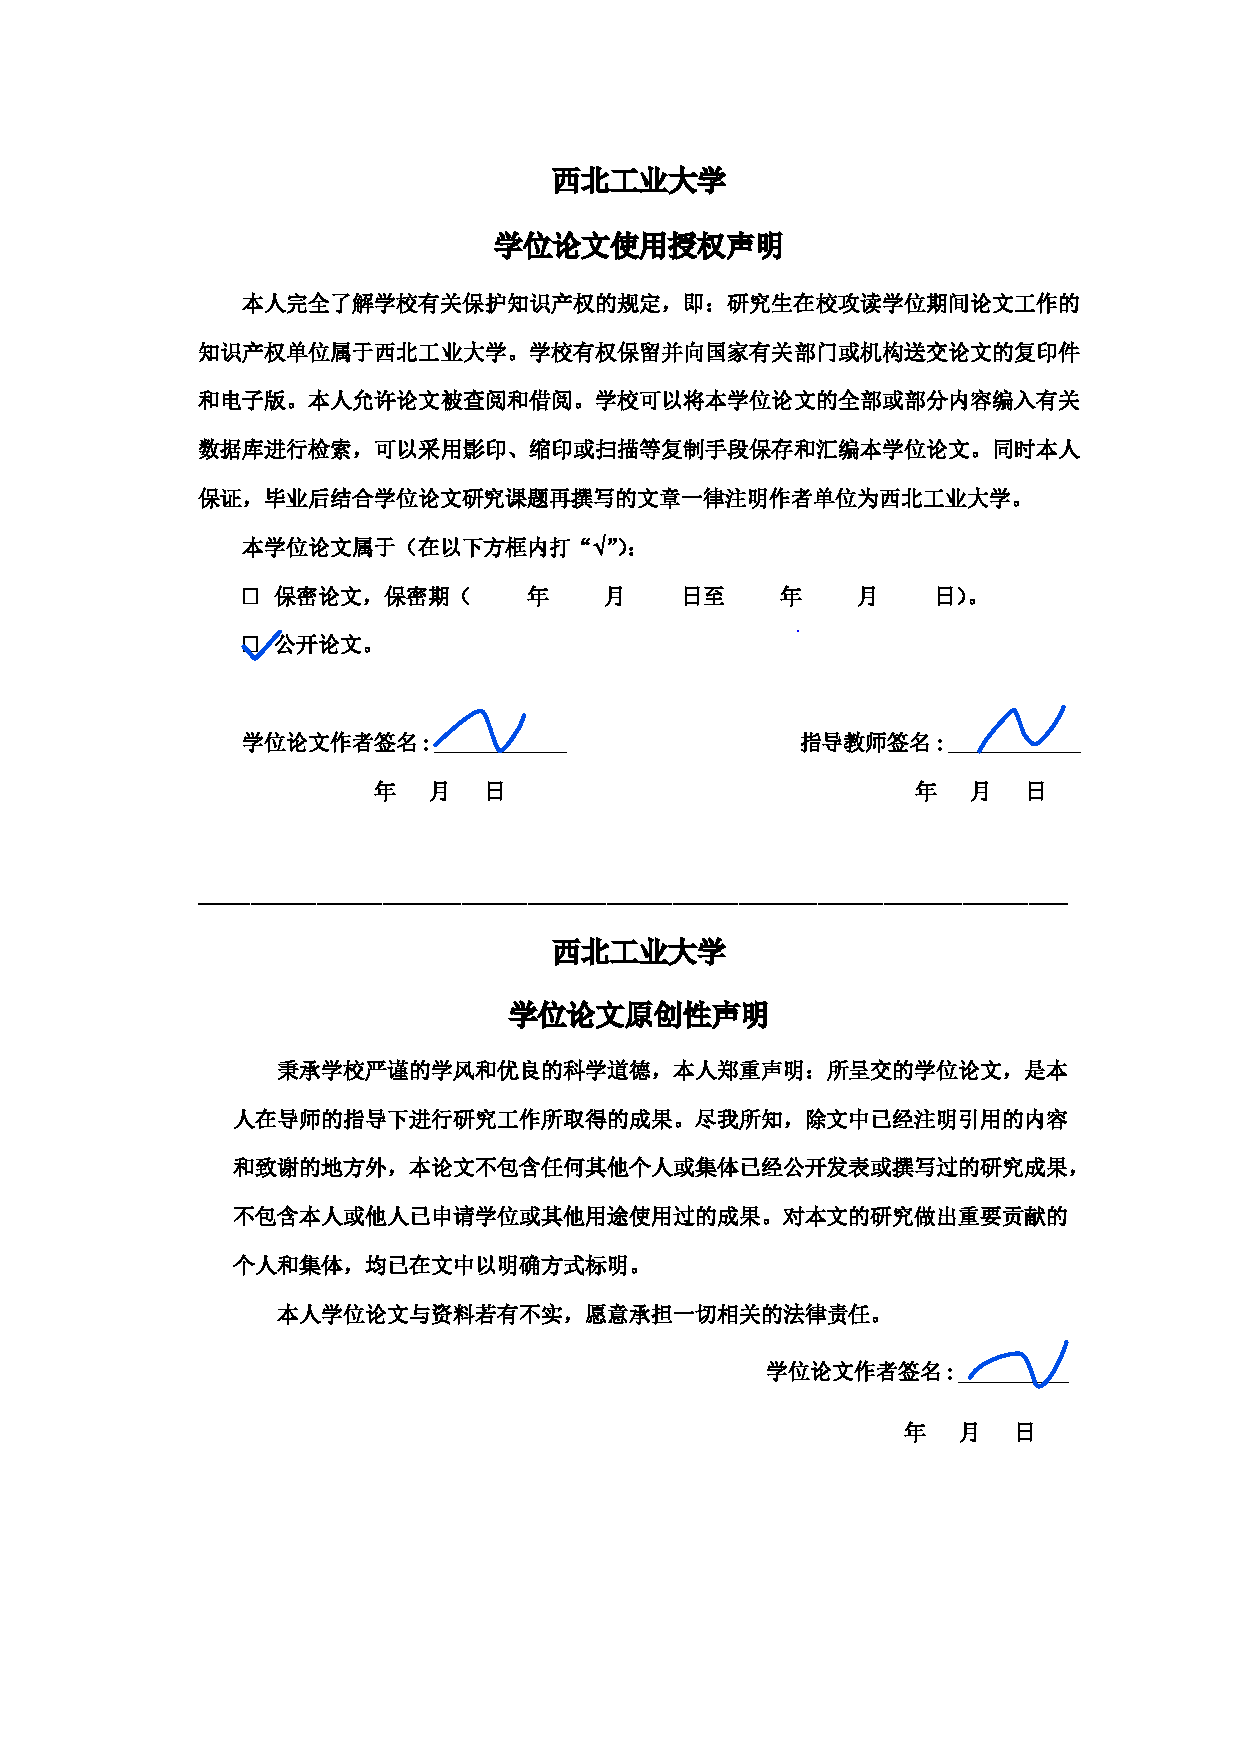
\includepdf[pages=1,fitpaper=true]{Resources/sign.pdf}

% 追加两页空白页
\clearpage
\thispagestyle{empty}\null\newpage
\thispagestyle{empty}\null\newpage

% 追加彩色封底页
\clearpage
\AddToShipoutPictureBG*{%
    \AtPageLowerLeft{%
        
\includegraphics[draft=false,width=\paperwidth,height=\paperheight]{Resources/acad_tail.jpg}%
    }%
}
\thispagestyle{empty}\null
\clearpage

%%=============================================================================%
%% 文档结束
%%-----------------------------------------------------------------------------%
\end{document}
%%=============================================================================%